\chapter{Hardware Subsystems}
\label{chap:hardware_subsystems}
In this chapter building blocks of the proposed system, each of which were separately prototyped to allow a good degree of parallelisation, are described. The driver software that makes each unit functional is also mentioned. We discuss the top-level software that brings these blocks together into a functional system in the chapter \ref{chap:system_software}.


\section{Monitoring Device}
The monitoring device is designed to be a simple device that acquires data from the sensors, stores the data and sends it to the base station when the ZigBee link is available. It contains a microcontroller, a set of sensors for data acquisition, a memory card to store data and a ZigBee module for wireless communications.

\begin{figure}
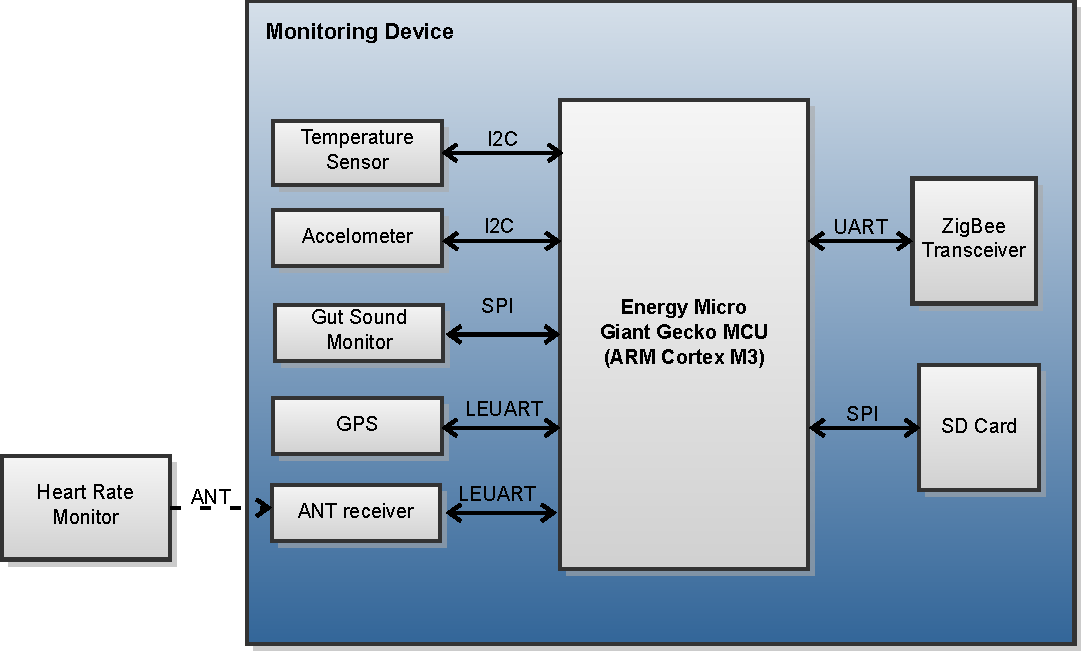
\includegraphics[width=\textwidth]{Images/MonitoringDeviceBlockDiagram}
\caption{Block Diagram: Monitoring Device}
\label{fig:monitoring_device_block}
\end{figure}

The following sub-chapters will discuss the implementation of each subcomponent of the monitoring device, shown in Figure \ref{fig:monitoring_device_block}, together with the properties of the hardware and how they map to the requirements of the project.


\subsection{The Microcontroller (MCU)}
As the monitoring device is required to be a battery-operated system that contain a number of diverse peripherals, choosing the right central processing unit was essential. Reviewing existing microcontrollers in the market we opted for an EFM32 Giant Gecko microcontroller from Energy Micro, which contains a 32-bit ARM Cortex M3 core and a set of on-chip peripheral interfaces. The EFM32 was considered to be a good match for the requirements, as shown in the table \ref{tab:microcontroller_properties}.

\begin{table}
\begin{tabular}{|m{0.45\textwidth}|m{0.45\textwidth}|}
\hline 
	\textbf{Device Properties} & 
	\textbf{Corresponding Requirements} \\ 
\hline
	\begin{itemize}
	\item up to 48 MHz high-frequency operation
	\end{itemize}&
	\begin{itemize}
	\item handle large data volumes from multiple sensors and audio
	\end{itemize} \\
	
\hline
	\begin{itemize}
	\item different levels of sleep
	\item fast wake up time (2 $\mu S$)
	\item 32.768 kHz low-frequency operation for sleep modes
	\item low energy periphals operational even in deep sleep modes
	\item DMA and PRS (Peripheral Reflex System) for acquiring data without waking up the processor core
	\end{itemize} &
	\begin{itemize}
	\item long battery life
	\item long periods of sleep
	\item low energy periodic sampling
	\end{itemize} \\
\hline
	\begin{itemize}
	\item 128 KB SRAM, 1MB flash memory
	\end{itemize} &
	\begin{itemize}
	\item ease of development
	\item suitable for overheads introduces by C++
	\end{itemize} \\
\hline
	\begin{itemize}
	\item 3 x USART with I2S support
	\item 2 x low energy UART (LEUART)
	\item 2 x I2C interfaces
	\end{itemize} &
	\begin{itemize}
	\item various interfaces for peripherals and sensors
	\end{itemize} \\
\hline
	\begin{itemize}
	\item 64-pin TQFP package
	\end{itemize} &
	\begin{itemize}
	\item ease of soldering (lack of BGA mounting equipment)
	\end{itemize} \\
\hline 
\end{tabular} 
\caption{Microcontroller properties}
\label{tab:microcontroller_properties}
\end{table}

Some of the more specialized properties of the microcontroller which give it advantages for our solution are briefly explained below:

\subsubsection*{Energy Modes and Low Energy Peripherals} The EFM32 microcontrollers offer four levels of sleep, and some special peripherals (called low energy or LE peripherals) that are able to keep functioning even in deep sleep modes. Of particular interest to us are the LEUART interface which while deeper sleep modes provide more energy savings, it also becomes more difficult to implement a reasonable level of active functionality. An overview of sleep modes and available peripherals in each is presented in table \ref{tab:microcontroller_modes}.

\begin{table}
\centering
\begin{tabular}{|l|l|m{6cm}|}
\hline
	\textbf{Energy Mode}&
	\textbf{Power consumption}&
	\textbf{Description}  \\ 
\hline
	EM0 &
	$200 \frac{\mu A}{MHz}$ &
	All peripherals active, CPU core active  \\ 
\hline
	EM1 &
	$50 \frac{\mu A}{MHz}$  &
	All peripherals active, CPU core sleep  \\ 
\hline
	EM2 &
	$1.2 \mu A$  &
	LEUART, LETIMER, I2C, RTC, LCD, PCNT, LESENSE, ACMP, OPAMP, USB active  \\ 
\hline
	EM3 &
	$0.9 \mu A$  &
	Full CPU and RAM retention, asynchronous external interrupts and I2C can wake up the device   \\ 
\hline
	EM4 &
	$20 nA$  &
	All functionality off, GPIO pin retention and wake up from GPIO interrupt  \\ 
\hline 
\end{tabular} 
\caption{Microcontroller energy modes}
\label{tab:microcontroller_modes}
\end{table}

\subsubsection*{Peripheral Reflex System (PRS)}
Using a signal producers - signal consumers concept, it is possible to make peripherals in the EFM32 microcontroller directly communicate with each other without involving the CPU. Thus, an action can be automatically triggered in peripheral A when an event occurs in peripheral B. This can be used to achieve more stable time-critical operations and less software overhead, as well as saving energy since the CPU does not have to intervene.

\subsubsection*{Direct Memory Access (DMA)} DMA allows blocks of data to be moved between RAM and peripherals without CPU intervention, thus freeing CPU resources and allowing longer periods of sleep, as well as offering stable high bandwidth memory transfers for operations like audio acquisition.

Further details of how the PRS, DMA and different sleep modes are used in the system is provided in chapter \ref{chap:system_software}


\subsection{Heart Rate Monitor (HRM)}
The heart rate is an important vital sign for any health monitor, although designing a portable device to acquire heart rate is not a trivial task. The issues of electrode placement, filtering out changes due to subject movement and processing the resulting ECG signal are challenging and time consuming. Another challenge specific to our project is acquiring both gut sounds and the heart rate; it is not possible to reliably acquire both signals from the same physical location so a wired microphone or electrode would have to be attached to the horse. 

To address both these problems, we chose an ANT wireless module that can be used with any ANT+ compatible heart rate chest strap, commercially available for both horses and humans. Attaching a separate heart rate monitor chest strap and transmitting heart rate information wirelessly solves the problems mentioned above and brings the additional advantage of making the system usable for humans.

\begin{table}
\centering
\begin{tabular}{|m{0.45\textwidth}|m{0.45\textwidth}|}
\hline 
	\textbf{Device Properties} &
	\textbf{Corresponding Requirements}  \\ 
\hline
	low power  &
	low energy periodic sampling  \\ 
\hline
	simple UART interface &
	ease of development \\
\hline
	can pair with a particular ANT+ HRM chest strap &
	monitoring multiple horses \\
\hline 
\end{tabular} 
\caption{Heart Rate Monitor properties}
\label{tab:hrm_properties}
\end{table}

\textbf{Interface:} \TODO{rephrase} LEUART with configurable baud rate, not lots of data so high BR does not make sense

\textbf{Driver:}
\TODO{talk about ANT driver:} LEUART, configure \& open network with wildcard id, establish connection \& rcv heart rate. search timeout \& disconnection \& pairing.


\subsection{Temperature Sensor}
5.1.3 Temperature Sensor
As with many other warm-blooded animals, body temperature can be a valuable tool for diagnosis in horses. While electronic temperature measurements are usually done by an element that comes into physical contact with the subject, doing temperature measurements in this manner on a moving horse is likely to cause fluctuations in the read values. This is the reason we preferred to use a contactless temperature sensor for our implementation. 

\TODO{Fix this} TMP006 [http://www.ti.com/lit/ds/symlink/tmp006.pdf] which is a contactless infrared temperature sensor from Texas Instruments was chosen for the project. 


\begin{table}
\centering
\begin{tabular}{|m{0.45\textwidth}|m{0.45\textwidth}|}
\hline 
	\textbf{Device Properties} &
	\textbf{Corresponding Requirements}  \\ 
\hline
	low power:
	\begin{itemize}
	\item 240-325 $\mu A$ during active conversion
	\item 90 $\mu A$ in sleep mode 
	\end{itemize}  &
	low energy periodic sampling  \\ 
\hline
	contactless temperature measurement &
	portable, mobile monitoring device \\
\hline
	passive (slave) device over I2C bus &
	advantageous for a system with lots of sensors, will not send and generate interrupts unless requested \\
\hline 
\end{tabular} 
\caption{Temperature Sensor properties}
\label{tab:temp_sensor_properties}
\end{table}

\textbf{Interface:} The TMP006 offers an SMBus-compatible interface, which is interoperable with I2C and was connected to the I2C interface on the microcontroller. Controlling device functionality and accessing measurement data is done via “write to register” and “read from register” commands. 

\textbf{Driver:} Our TMP006 driver configures device sleep state and conversion rate by writing values to the appropriate registers (TODO insert reference to TMP006 datasheet). The temperature measurement is provided by reading the two registers which contain the voltage generated by the thermopile and the die temperature. The temperature of the object can be calculated from these two data. However this calculation involves heavy floating point arithmetic and it is rather inefficient on the microcontroller. Therefore, the “raw” temperature reading consisting of these two values is not processed on the monitoring device any further but sent to the base station, whose ARM11 core is much more efficient at handling this calculation. 


\subsection{GPS}
A popular peripheral in many consumer devices today, GPS (Global Positioning System) allows tracking the position of a sensor in terms of global coordinates. While not immediately useful for clinical purposes, the ability to track the location of horses on this level can be beneficial if recording of movements or activity recognition [TODO ref High Classification Rates for Continuous Cow Activity Recognition using Low-cost GPS Positioning Sensors and Standard Machine Learning Techniques.]  is desired over a longer period of time in a larger area (for free-roaming horses or other animals). 

Commercial drop-in GPS modules are available and straightforward to use, but power consumption while searching limits the possibilities for a battery-powered system with energy efficiency focus. We chose a UP500 GPS module from Fastrax \footnote{\url{http://www.fastraxgps.com/products/gpsantennamodules/500series/up500/}}
for our project. UP500 is a GPS receiver module with embedded antenna offered in a very small package, and offers significant power savings by providing an option to save satellite data to RAM while still being able to wake up from this state and get a position fix within a few seconds (called a “hot start”). 

\textbf{Interface:} The UP500 with the microcontroller via UART and uses a baud rate of 9600 (8 data bits, 1 stop bit, no parity). The Low Energy UART (LEUART) peripheral on the EFM32 was used for this connection, which can receive data at low baud rates even while in deep sleep mode (down to EM2).

\textbf{Driver:}
\begin{itemize}
\item{Data acquisition:}
For maximum energy efficient operation, the GPS driver configures the GPS module to use LEUART interface with DMA. DMA transfers incoming NMEA messages into a fixed size buffer when new data is available. The LEUART module is configured to generate an interrupt whenever it receives the newline character (0x0A). Since every NMEA message ends with a newline, an interrupt is generated every time a complete message is received, and the contents of the DMA buffer are copied to another internal buffer for processing at a later time.

\item{Parsing NMEA messages:} \TODO{} simple string parsing, comma delimited fields,NMEA message types GPRMC and GGPA are handled
\begin{itemize}
\item output: valid position fix, latitude and longitude
\end{itemize}

\item{Sleep mode:} The UP500 does not have a dedicated sleep pin, but once satellite data has been acquired it is possible to put the device into a sleep-like mode where the power consumption becomes quite low. This is done by turning off the power to the $V_{cc}$ supply pin, while keeping the $V_{bat}$ supply pin active. By keeping ephemeris data in RAM, the GPS is thus able to establish the position quickly when the $V_{cc}$ supply is reinstated. Switching the $V_{cc}$ supply is done via a transistor attached to a GPIO pin, consult section \TODO{} for more details.
\end{itemize}


\subsection{Accelerometer}
In addition to the location tracking capabilities provided by the GPS, it can be useful to measure smaller movements with higher precision. Accelerometer data collected in this manner can be used to detect lameness and injuries. The particular challenge for using an accelerometer in our system was the high sampling rate necessity - the collected acceleration data will not be useful at low sampling rates\footnote{\TODO{find a good citation for this}}. While high sampling rate itself is not a problem for the EFM32 microcontroller, it conflicts with low energy periodic sampling - if the microcontroller has to poll the device for new data at a high frequency, it will not have a lot of time to sleep. An accelerometer that contains an on-chip buffer can remedy this problem; the MCU can simply enable sampling, go back to sleep, and wake up when the desired number of samples have been acquired to read them from the sensor’s own buffer.

We chose the 3-axis  ADXL350 \footnote{\url{http://www.analog.com/en/mems-sensors/mems-accelerometers/adxl350/products/product.html}} digital accelerometer from Analog Devices for the project. It is capable of measuring acceleration in the ranges ±1g, ±2g, ±4g or ±8g and it has a FIFO buffer which allowed us to implement the scheme discussed in the previous paragraph.

\begin{table}
\centering
\begin{tabular}{|m{0.45\textwidth}|m{0.45\textwidth}|}
\hline 
	\textbf{Device Properties} &
	\textbf{Corresponding Requirements}  \\ 
\hline
	.
	\begin{itemize}
	\item Ultralow power: $45 \mu A$ in measurement mode and $0.1 \mu A$ in standby mode
	\item FIFO buffer can hold up to 32 samples
	\end{itemize} &
	low energy periodic sampling  \\ 
\hline 
\end{tabular} 
\caption{Accelerometer Sensor properties}
\label{tab:accelerometer_properties}
\end{table}

\textbf{Interface:} Similar to the TMP006, the ADXL350 is interfaced through the I2C bus; controlling device functionality and accessing measurement data is done via “write to register” and “read from register” commands. 

\textbf{Driver:} ADXL350 supports both SPI and I2C interfaces. In this project, it is used in I2C mode. The accelerometer offers a 32-level FIFO which has 4 modes of operation configured by control registers: Bypass, FIFO, Stream and Trigger Mode. The driver configures the FIFO in Bypass Mode which disables the FIFO. The 4-phase scheme (\TODO{I don’t know how to refer this}) is applied for power management. 


\subsection{Gut Sound Monitoring}
One key feature of the desired Equine Health Monitoring System is the possibility to acquire and record sounds coming from horses guts which can come very useful for diagnosis of multiple health disorders in the digestive tract of the animal under observation.

As it was mentioned in chapter \ref{chap:research} listening the gut is a common task performed by a specialist during a regular physical examination. This is done by placing a stethoscope in several parts of the animal’s trunk. Intermittent noises that will repeat every 15-30 seconds will be detected in a healthy animal. The specialist will monitor this sounds for an interval of 4-5 minutes. The aim of the designed system is to record and store those sounds which will eliminate the need for a physical examination in situ by a specialist.


\subsubsection{Audio acquisition requirements}
During the background research phase the group realized that a comprehensive digital database of recordings of gut noises is regrettably not available on the web. And despite of different attempts the group was not able to obtain an audio sample of good quality. Hence a proper signal profiling and characterization could not be performed. The quality parameters for audio samples were defined to meet the hearing capabilities of the final human user (a veterinary specialist) instead of the characteristics of the signal source.
The recording of audio samples implies two challenges that are not shared by the other sensors in the system.
\begin{itemize}
\item \textbf{Real time constraints:} Audio acquisition is a real time..... need periodic accurate time sampling.. 
\item \textbf{High data rate:} memory...
\end{itemize}

\begin{align*}
\centering
datarate_{audio}&=f_{sampling} * \frac{Bits}{Sample}* t_{recording} \\
datarate_{audio}&=8000 Hz * 16 \frac{Bits}{Sample}* 240s
\end{align*}


\subsection{Component selection justification}
The component ADMP441 from Analog Devices was chosen for the audio acquisition. This single-chip MEMS (Micro Electro Mechanical System) microphone provides very convenient characteristics which are summarized in the following table.

\begin{table}
\centering
\begin{tabular}{|m{0.45\textwidth}|m{0.45\textwidth}|}
\hline 
	\textbf{Device Properties} &
	\textbf{Corresponding Requirements}  \\ 
\hline
	Single chip solution: MEMS sensor, signal conditioning, analog-to-digital converter, antialiasing filters, power management
	&
	Ease of integration. No need for extra components (codecs/amplifiers)\\ 
\hline 
	I2S digital interface 
	&
	Ease of integration, industry standard \\
\hline
	Low voltage supply and current consumption: \newline
	3.3 Vdd \newline
	Normal mode: 2.5 mA \newline
	Standby mode: 0.8 mA \newline
	Power down mode: 4.5 uA
	&
	Low energy consumption \\
\hline
	16-24 bit samples \newline
	High SNR: 61 dBA \newline
	High sensitivity: −26 dBFS \newline
	Flat frequency response from 60 -15000 Hz
	&
	Audio quality suitable for the project scope, high intelligibility \\
\hline
	Small size: 4.72mm × 3.76mm × 1mm smd package 
	&
	Low weight, portability
\\\hline	
\end{tabular} 
\caption{MEMS microphone properties}
\label{tab:microphone_properties}
\end{table}

A scheme of the required signal processing stages in general digital audio system are shown in figure \TODO{Ref}.
The first stage consists of a transducer or microphone that will react to the sound waves in the air and produce an electric signal. This electrical signal has to be properly conditioned for the following steps, this includes amplification and filtering. The analog signal needs to be sampled and quantized. This will generate a set of binary words corresponding to each sample. Commercially available Analog to Digital Converters will provide a serial flow of bits, this is known as pulse code modulation (PCM).

\paragraph*{Microphone placement:} TODO: describe the plastic coupling piece and the stethoscope head, which enable the sensing of gut sounds. Add picture of the device.

\paragraph*{Interface:} The ADMP44 chip uses I2S protocol as interface. I2S, also known as Inter-IC Sound, Integrated Interchip Sound, or IIS, is an serial bus interface standard used for connecting digital audio devices together. It is used to transmit PCM (Pulse Code Modulation) audio data.

\paragraph*{Driver:} The I2S standard is supported by the microcontroller’s Universal Synchronous Asynchronous Receiver Transmitter (USART) which simplified the implementation of the driver for this sensor.
Driver: The implementation of a driver for fetching audio data was a rather complex task. 
Normally specialized electronic devices such as Digital Signal Processors (DSP) and audio codecs are employed to satisfy the requirements of recording, storage and processing. But in this project, in order to keep a minimal design and low power consumption no extra processing units were added to handle the audio functionalities and the general purpose microcontroller was used instead. 
Advanced hardware features of the microcontroller are used to perform this tasks as it will be 
 explained in the following sections.
DMA... ping pong.

In order to provide a permanent input of audio samples without interruptions double buffered DMA transactions to move data from the USART to the final storage device were used. This strategy is explained in detail in section XX TODO: add section. 




\subsection{Data Storage}
Relatively low throughput of ZigBee link between the base station and the monitoring devices makes gut sound streaming inconvenient considering the amount of audio data produced. \TODO{}: Here we can quote amount of audio\ldots. One possible solution was to stream a smaller amount of data and record a longer audio data into an on-board storage element. Therefore, a microSD card was incorporated into the system. 

SD Card solution provides two other benefits to the system besides complementing the limits of wireless streaming. The SD Card can be used to save data collected from all sensors when the base station is out of reach. This way the sensor data is not lost when there is no connection between the base station and the monitoring device. Also, it can be removed by the user to copy the data when needed, since a wide range of devices are SD card compatible.  

SD Cards are based on flash memory technology. They support 3 communication modes: SD 1-bit, SD 4-bit and SPI mode\footnote{\url{http://alumni.cs.ucr.edu/~amitra/sdcard/Additional/sdcard_appnote_foust.pdf}}. 

In SD 1-bit mode, the data is transferred over 1-bit wire in a synchronous serial fashion. SD 4-bit protocol is the same as SD 1-bit protocol except that bulk data transfer is done over 4-bit bus. SD 4-bit mode can provide speed benefits over SPI mode. However it is not recommended in software solutions since it requires CRC calculation for each of the four wires and may result in a big computational effort. Also, accessing the complete SD Card Specifications to build an SD standard device requires licenses from SD Card Association\footnote{\url{https://www.sdcard.org/developers/howto/}}. Therefore, in this project, the card is used in SPI mode. 

\TODO{Check this:}TODO: Check this (“If your company is planning to manufacture or have manufactured SD standard devices  (eg. cell phones, cameras or computers) or SD ancillary products (eg. adapters or SD I/O cards), your company is required to:”, I think using SD bus is “manufacturing an SD standard device”)

To implement microSD prototype system, an existing FAT file system and a low-level disk interface module were used. The card was connected to one of the SPI interfaces of the microcontroller. MicroSD cards support up to 208 MHz clock frequency [TODO citation]. The clock system of the Energy Micro microcontroller allows maximum SPI bit rate to be at half speed of the source clock in master mode \TODO{Citation: EFM32\_GG Ref}. Theoretically, SPI clock can be up to 24 MHz when the source clock is set to 48 MHz. However, there is an upper speed limit caused by delays of inputs and outputs of the microcontroller which is not specified by the manufacturers\footnote{\url{http://forum.energymicro.com/topic/288-microsd-card-spi-baudrate/}}. Our microSD driver sets SPI clock speed at \TODO{X} Mhz at which it operates safely.   


\section{Wireless Interfaces}
\subsection{Data transmission - ZigBee}
Because of the decision to design a distributed system that transmits data wirelessly between monitoring devices and the base station, it was necessary to come up with a customized stable wireless communication path. As discussed in section \ref{sec:wireless_connection} the ZigBee protocol was chosen for the wireless communication between the base station and the monitoring devices.

As ZigBee is an open standard there are multiple vendors offering devices implementing the protocol. Because of the widespread use in homebrew electronic projects we decided to use devices by Digi which offer a whole ZigBee based product line called XBee. 

The main advantage was that the prototyping could be sped up due to availability of breakout boards, and XBee to USB converters (figure \ref{fig:xbee_prototyping_interfaces}). This allowed to implement, test and debug the software module for wireless communication on a normal computer before porting it to the embedded system.

\begin{figure}
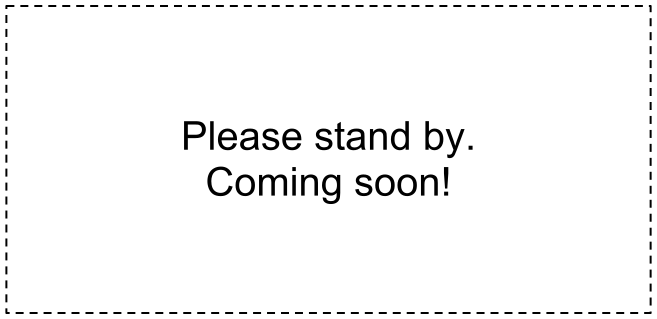
\includegraphics[width=\textwidth]{Images/dummy}
\caption{XBee prototyping interfaces}
\label{fig:xbee_prototyping_interfaces}
\end{figure}

The wireless software module uses an existing open-source software library to handle the low level communication with the XBee hardware, and adds an object oriented interface as well as utility classes that allow to use and control the wireless connection at a high abstraction level. More details on the design of the software module are given in section \ref{sec:wireless_communication_software}


\subsection{Communication with Heart Rate Monitor - ANT}
\TODO{Not yet written}


\section{Base Station}\begin{figure}
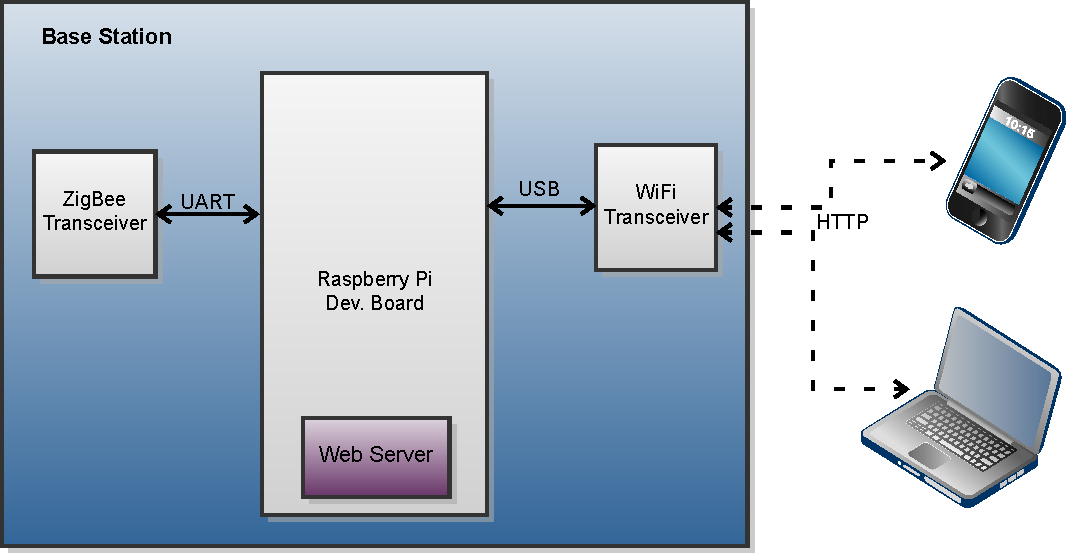
\includegraphics[width=\textwidth]{Images/BaseStationBlockDiagram}
\caption{Block Diagram: Base Station}
\label{fig:block_base_station}
\end{figure}

The base station collects data from the monitoring devices, stores this data in a database and makes it available and via a webserver running on the device itself. The advantage of using a website to provide access to the collected data is the support for a variety of devices with web access. In addition, it compensates disadvantage of the short range low data-rate ZigBee connection making the data accessible from anywhere.  


\subsection{Hardware platform}
The base station acts as a bridge between the “proprietary” monitoring stations and the end user, who wants an easy way to access the data that is collected by the system. The challenges for the base station lay mainly in the software domain. The only requirements that exist for the platform is that it has a to be able to interface an XBee device, a WLAN transceiver and provide means for mass data storage. 

For these reasons the decision was made, that an existing hardware platform would be used to implement the base station. The choice fell on the Raspberry Pi which provides a number of positive implications that are listed in table \ref{tab:raspberry_capabilities}.


\subsection{Raspberry Pi}
\begin{table}
\centering
\begin{tabular}{|l|m{6cm}|}
\hline
	Price &
	35£   \\ 
\hline
  	Software &
  	Raspberry can run a Debian based distribution, which gives access to a huge set of open-source programs and libraries  \\ 
\hline
	Connectivity &
	Features an ethernet port, USB host capabilities and HDMI output that could be used to attach a display to the base station  \\ 
\hline
	Extendability / GPIP  &
	20 GPIO pins, support for I2C, SPI, Serial  \\ 
\hline
	Storage &
	SD-Card slot with support for cards up to 64GB  \\ 
\hline
	Power consumption &
	Very low, between 1.5 and 2 Watt \\ 
\hline
 	Size &
 	Very small form factor (85.6mm x 56mm)  \\ 
\hline 
\end{tabular} 
\caption{Raspberry Pi capabilities}
\label{tab:raspberry_capabilities}
\end{table}

In summary it can be said that the Raspberry Pi is very well suited for rapid development of embedded systems, as long as they are not supposed to run on battery. It offers the convenience of developing software in a Linux environment while giving direct access to low level I/O capabilities for interfacing custom hardware.

\subsection{XBee}
As mentioned in section \ref{sec:wireless_connection} we use of XBee devices to implement the ZigBee network for data transmission between monitoring devices and the base station. These devices are widely-used in (homebrew) electronic projects, and they have the advantage that a Raspberry compatible XBee adapter board already exists. The adapter goes by the name of Slice of Pi and is shown in figure \ref{fig:xbee_prototyping_interfaces}.
